% Visualizing a quotient G/N as fibers: G is drawn as 6 vertical
% "columns", each column being a coset (the dots are elements of the
% coset). Each column collapses downward (double-arrow) to a single
% point in the quotient Q below.
% Source: book/tex/H113/quotient.tex (§ Cosets and modding out).
\documentclass[border=2mm]{standalone}
\usepackage{tikz}
\begin{document}
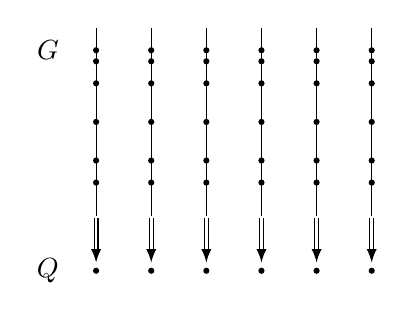
\begin{tikzpicture}[>=latex, scale=0.7]
  \foreach \i in {1,...,6} {
    % Vertical "column" representing a coset.
    \draw (\i,0) -- (\i,3.4);
    % Six points (representative elements within the coset).
    \fill (\i,0.6) circle (1.6pt);
    \fill (\i,1)   circle (1.6pt);
    \fill (\i,1.7) circle (1.6pt);
    \fill (\i,2.4) circle (1.6pt);
    \fill (\i,2.8) circle (1.6pt);
    \fill (\i,3)   circle (1.6pt);
    % Double-arrow downward from G to Q.
    \draw[double, double distance=1pt, ->, line width=0.4pt]
      (\i,-0.05) -- (\i,-0.85);
    % Image of the coset in Q (one point per coset).
    \fill (\i,-1) circle (1.6pt);
  }
  % Labels for G and Q, on the left of each row.
  \node[left] at (0.5,3) {$G$};
  \node[left] at (0.5,-1) {$Q$};
\end{tikzpicture}
\end{document}
